 
Nowadays there is a growing interest in the 3D scene reconstruction field, due to the increasing computational power and the reduction of 
the costs of the capturing devices. There are many approaches to deal with this problem, for example 3D reconstruction 
from a video, from a set of images taken with an unknown camera and orientation, using active devices that project patterns of light into 
the scene, lasers, etc. 

In 3D reconstruction an important part of the problem depends of the intrinsic 
device characteristics (noise, resolution, frame-rate, etc.), the scene, the object being captured, illumination, camera location and position, etc. All these 
factors lead to different instances of the problem, difficulting the comparison and limiting the use of a common dataset. There are several datasets 
available on internet, such as for example \cite{sturm12iros},  \cite{LaiBRF11} and \cite{ShottonGZICF13}.

The researchers can estimate system performance comparing the generated 3D model with some 
ground truth model obtained with a high precision laser scanner, but is not always possible to have a ground truth model, because lasers scanners 
are expensive equipments. Due to this, it is common to measure the performance
 comparing some result obtained at an intermediate step of the reconstruction process with a ground truth measure, 
such as sensor trajectory.   

%done
Reconstruction from a set of photographs without human assistance is performed in \cite{jan}, they demonstrated the first system able to deliver dense geometry for Internet scale photo collections with millions of images of an entire city within the span of a day on a single PC. They used appearance-based clustering in multiple CPU and GPU cores 
in order agrupate images corresponding to the same site, using gist features for each image along with a RGB
descriptor in order to maintain color information. They also used geo-location information available for some  images. 
Then in each one of the clusters they performed 3D reconstruction using only the images with mutually consistent epipolar 
geometry. Using millions of images from one city they generated thousands of 3D models of buildings. See figure \ref{fig:jan}. 


\begin{figure}[h!]
\begin{center}
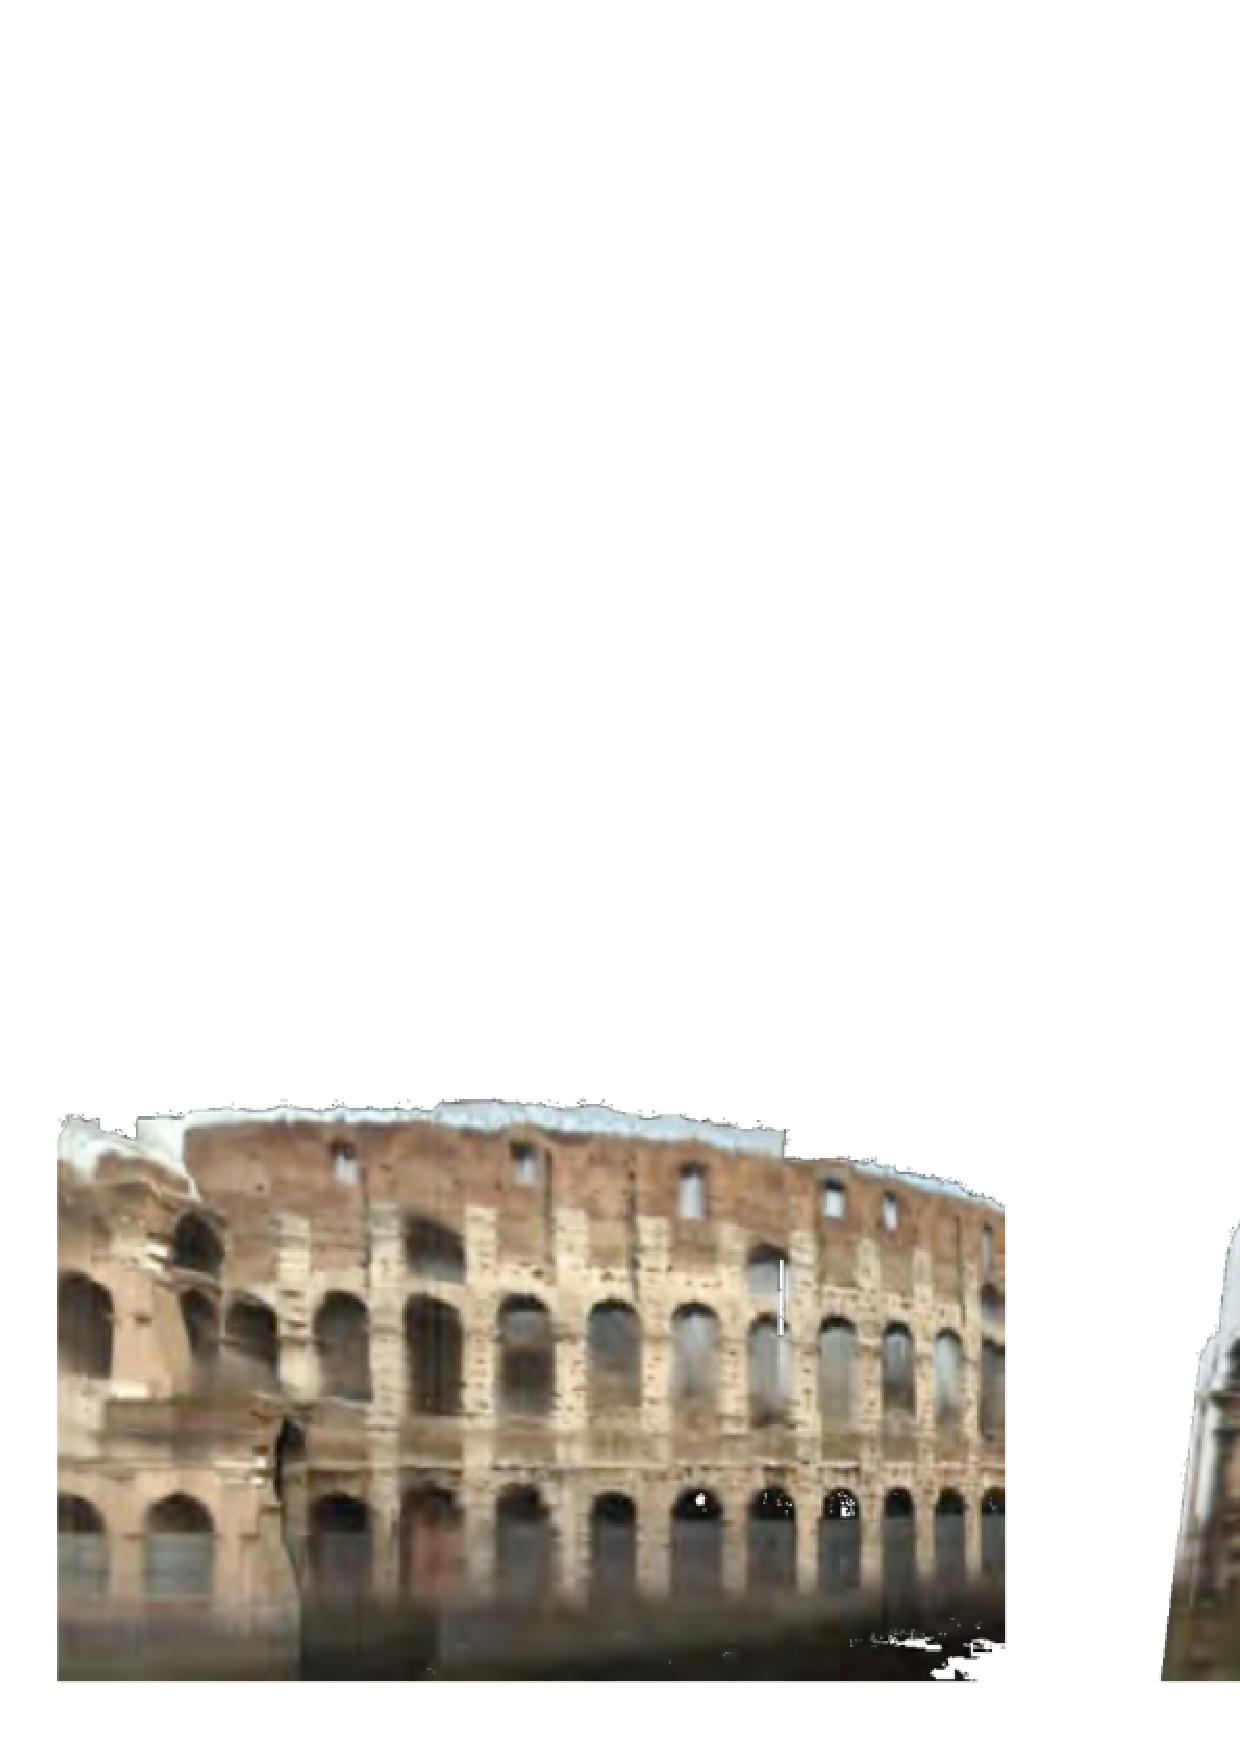
\includegraphics[scale=0.25]{images/jan}
\caption{Reconstructed 3D buildings in less than 24 hr. using 2.8 million and 2.9 million of images respectively.}
\label{fig:jan}
\end{center}
\end{figure}

%done
In \cite{guangyu} a hybrid approach is used, combining a Time of Flight (ToF) camera and a grayscale camera in order to perform the reconstruction. 
The data acquisition is made rotating the object in front of the camera with a black background behind it, then they use 
Scale Invariant Feature Transform (SIFT) to find 2D feature correspondences and perform an initial alignment between two consecutive frames, this alignment is 
then improved with ICP algorithm. They use a 3D laser scanner in order to obtain a ground truth, obtaining a difference around of 1\% 
between their reconstructed
 models and the 3D laser models. See figure \ref{fig:guangyu}.




\begin{figure}[h!]
\begin{center}
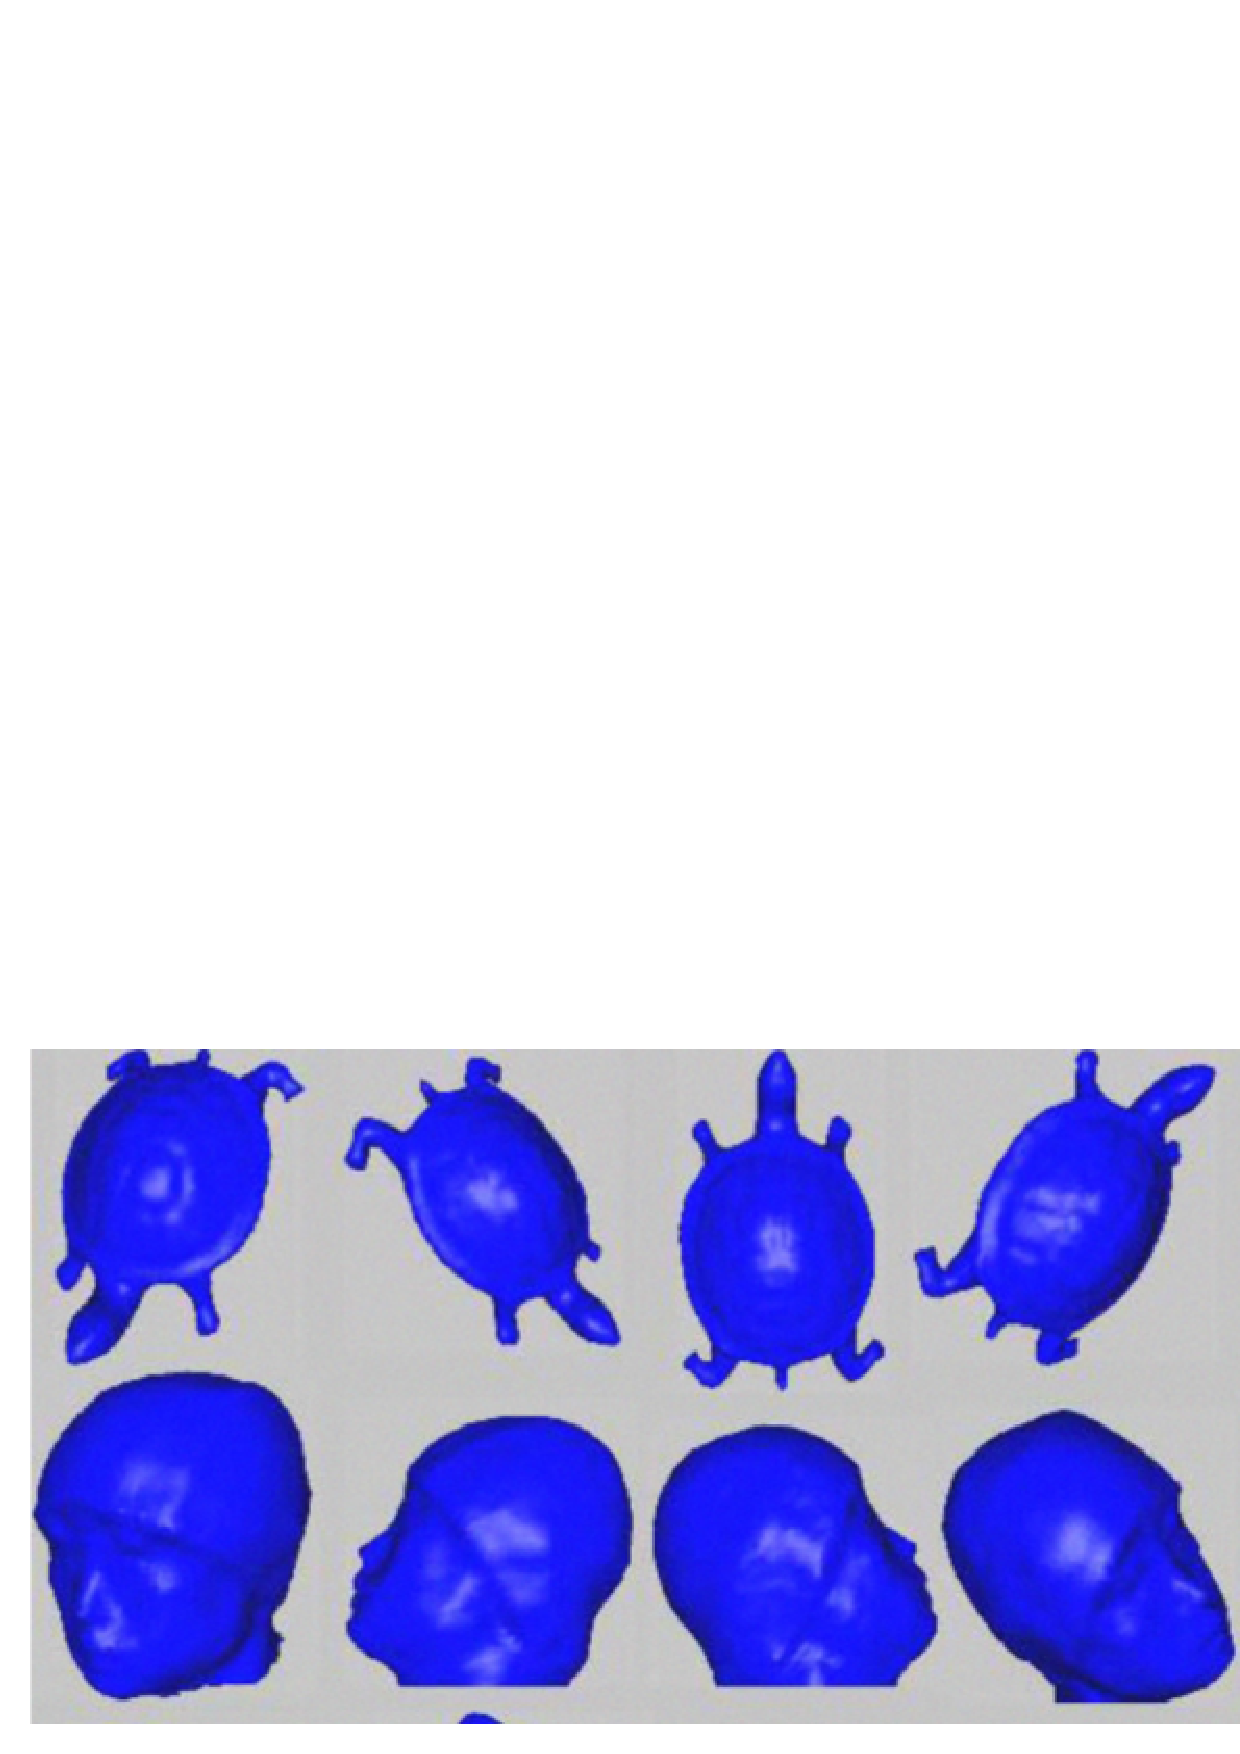
\includegraphics[scale=0.38]{images/guangyu}
\caption{3D Reconstruction of a human head and an object using ToF and RGB camera.}
\label{fig:guangyu}
\end{center}
\end{figure}

%done
In \cite{may2009} a ToF camera is used in combination with an industrial robot arm (KUKA KR 16) in order to register an indoor scene,
they use an improved version of the ICP algorithm called ICP Frustum, where at each iteration the points that are not overlapping with the previous frame are removed. The industrial robot arm is used to move the camera and get a ground truth camera path to evaluate the performance of their ICP algorithm. 



%revisar nuevamente
 Indoor scene reconstruction is made in \cite{henry} using an RGB-D camera. RGB-D cameras are sensing systems that capture RGB images
 along with per pixel depth information. They use the ICP algorithm to calculate the camera location, using information from 
the depth camera and  rich visual
 features captured by the RGB camera, along with Random Sample Consensus (RANSAC) verification. They use surfels \cite{pfister} to represent the scene. See figure \ref{fig:henry}.

\begin{figure}[h!]
\begin{center}
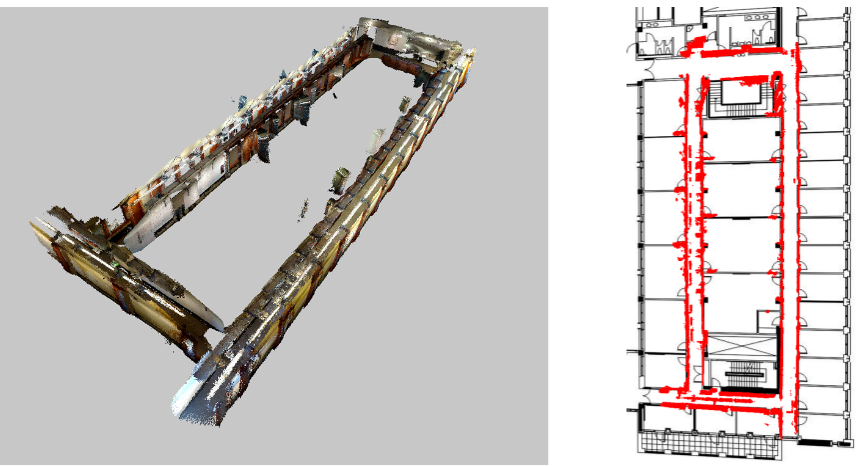
\includegraphics[scale=0.29]{images/henry}\caption{Reconstructed 3D big indoor space.}
\label{fig:henry}
\end{center}
\end{figure}

%
In \cite{cui} a ToF camera is used to reconstruct 3D objects. A combination of 3D superresolution method with a 
probabilistic scan alignment (iterative expectation maximization) approach that takes into account the sensor's 
noise characteristics is used. Their method is not in real time and the resulting models contains undesirable 
artifacts due to  the noise of the captured depth maps, they use a low resolution device (176x144), 
improving the resolution using a superresolution method. They captured a ground truth model with a laser 3D scanner, 
obtaining differences below 1 cm in most areas between their model and the ground truth model. Their scanning 
procedure does not allow a free movement around the object, the object must be at the center of view of the camera 
and the distance between the object and camera must be almost constant. See figure \ref{fig:cui}.

\begin{figure}[h!]
\begin{center}
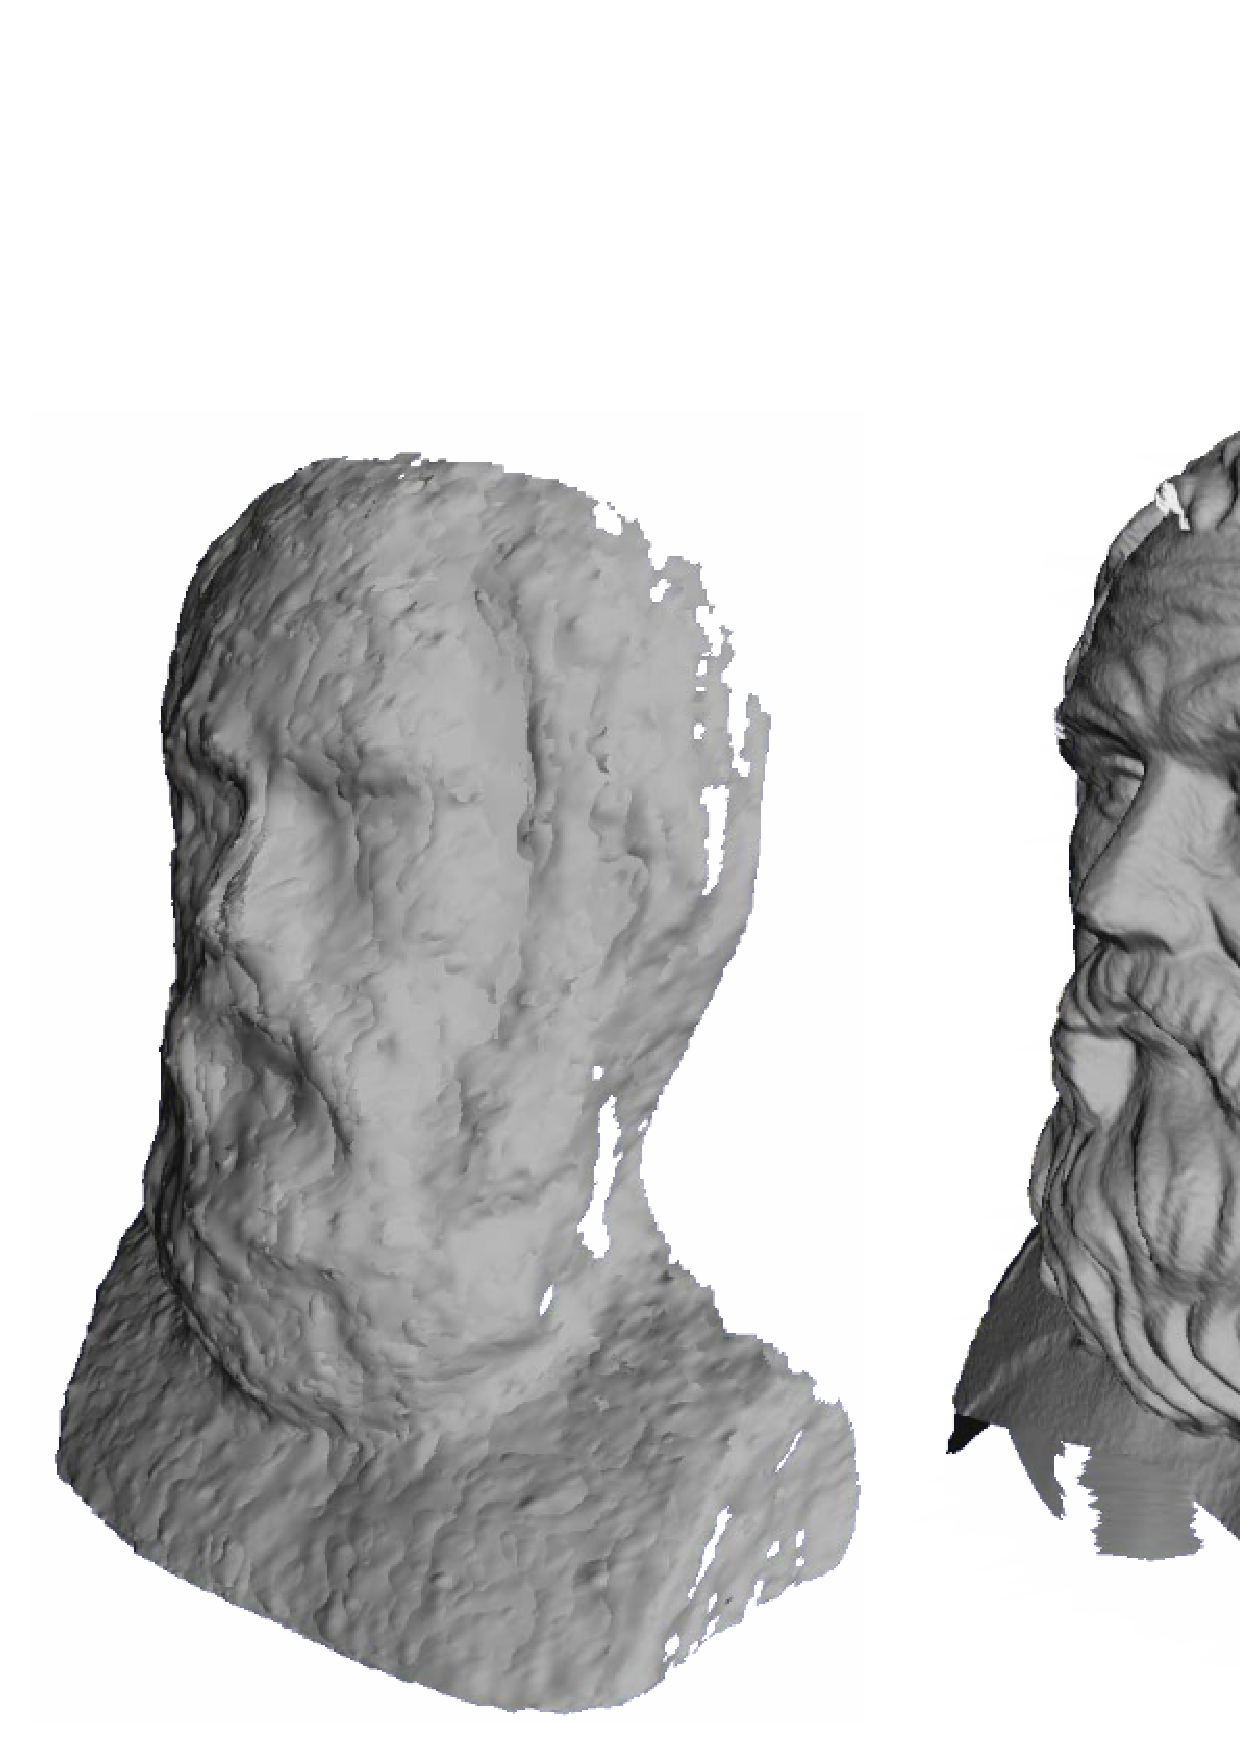
\includegraphics[scale=0.23]{images/cui}
\caption{ToF reconstruction, laser reconstruction and error plot.}
\label{fig:cui}
\end{center}
\end{figure}

In \cite{huhle} a ToF camera and a RGB camera are used to generate a 3D model, they combine geometric and color information, 
using SIFT to determine matching features between the RGB images, 
this 2D points are then converted into 3D points using the depth information. They use  Normal Distributions Transform (NDT) \cite{biber03} to exploit the geometrical 
information. NDT is a registration algorithm that use a different principle than ICP, it does not need point matches 
between successive frames. NDT build a grid on the 2D depth image, calculating the mean and the covariance matrix for each 
 cell. The respective normal distributions are used to estimate the probability of any transformed point $T(x_i)$ to fall 
inside some cell. Then they define a function that depends on the RGB matching features and NDT, in order to find the desired 
rigid transformation.

 
%done
A very interesting work is made in \cite{izadi}(figure \ref{fig:izadi}), they use a low cost RGB-D camera (Kinect) in order to perform
the 3D reconstruction, using the ICP algorithm  and a volumetric representation, with a GPU in order to 
achieve real time reconstruction. The camera can move freely around the scene and the reconstruction grows in detail 
as new depth measurements are added. They apply color textures to the reconstructed scene obtaining very 
realistic models. Their system is able to perform rigid body collisions 
simulations during the reconstruction, allowing thousands of virtual particles to interact with the scene. Also, a 
user can interact with the scene during the reconstruction process. This was one of the most advanced low cost 
reconstruction systems for its date, due to its unique features. A precursor work of \cite{izadi} is \cite{Newcombe10livedense}, where 
 just an RGB camera is used, obtaining impresive results. In order to perform the reconstruction a set of frames around 
a reference frame are used, generating a local model. Then a global model is generated merging all the local reconstructions.
The global model is deformed and gets more detail with every new local model added. This work not just confronted 
the geometrical problem of aligning several clouds of points, it also had to generate the point clouds from RGB images.

A more recent work is \cite{Steinbrucker_2013_ICCV} where large indoor reconstructions were performed 
with RGB-D data, using a multi-scale octree representation of a signed distance function and a GPU to work in real time. They use 
the same scene representation than  \cite{izadi}, but a different alignment process. Instead of aligning the frames to the reconstructed 
model, they use dense alignment between consecutive frames, 
using both depth and intensity images with an error  minimization approach. They claim that their alignment procedure is less prone to drift than
 the used by \cite{izadi}. A database was used, exposing quantitative results and comparisons. Another work 
extending the \cite{izadi} proposal is \cite{Whelan13} where visual odometry is used along with a volumetric representation. In \cite{KerlSC13} also RGB-D data with dense alignment was used, they integrated keyframes to the process in order to reduce drift. Other 
interesting works are \cite{bylow-sturm-etal} and \cite{quadrocopter} they use a signed distance function to represent scene geometry. 


\begin{figure}[h]
\begin{center}
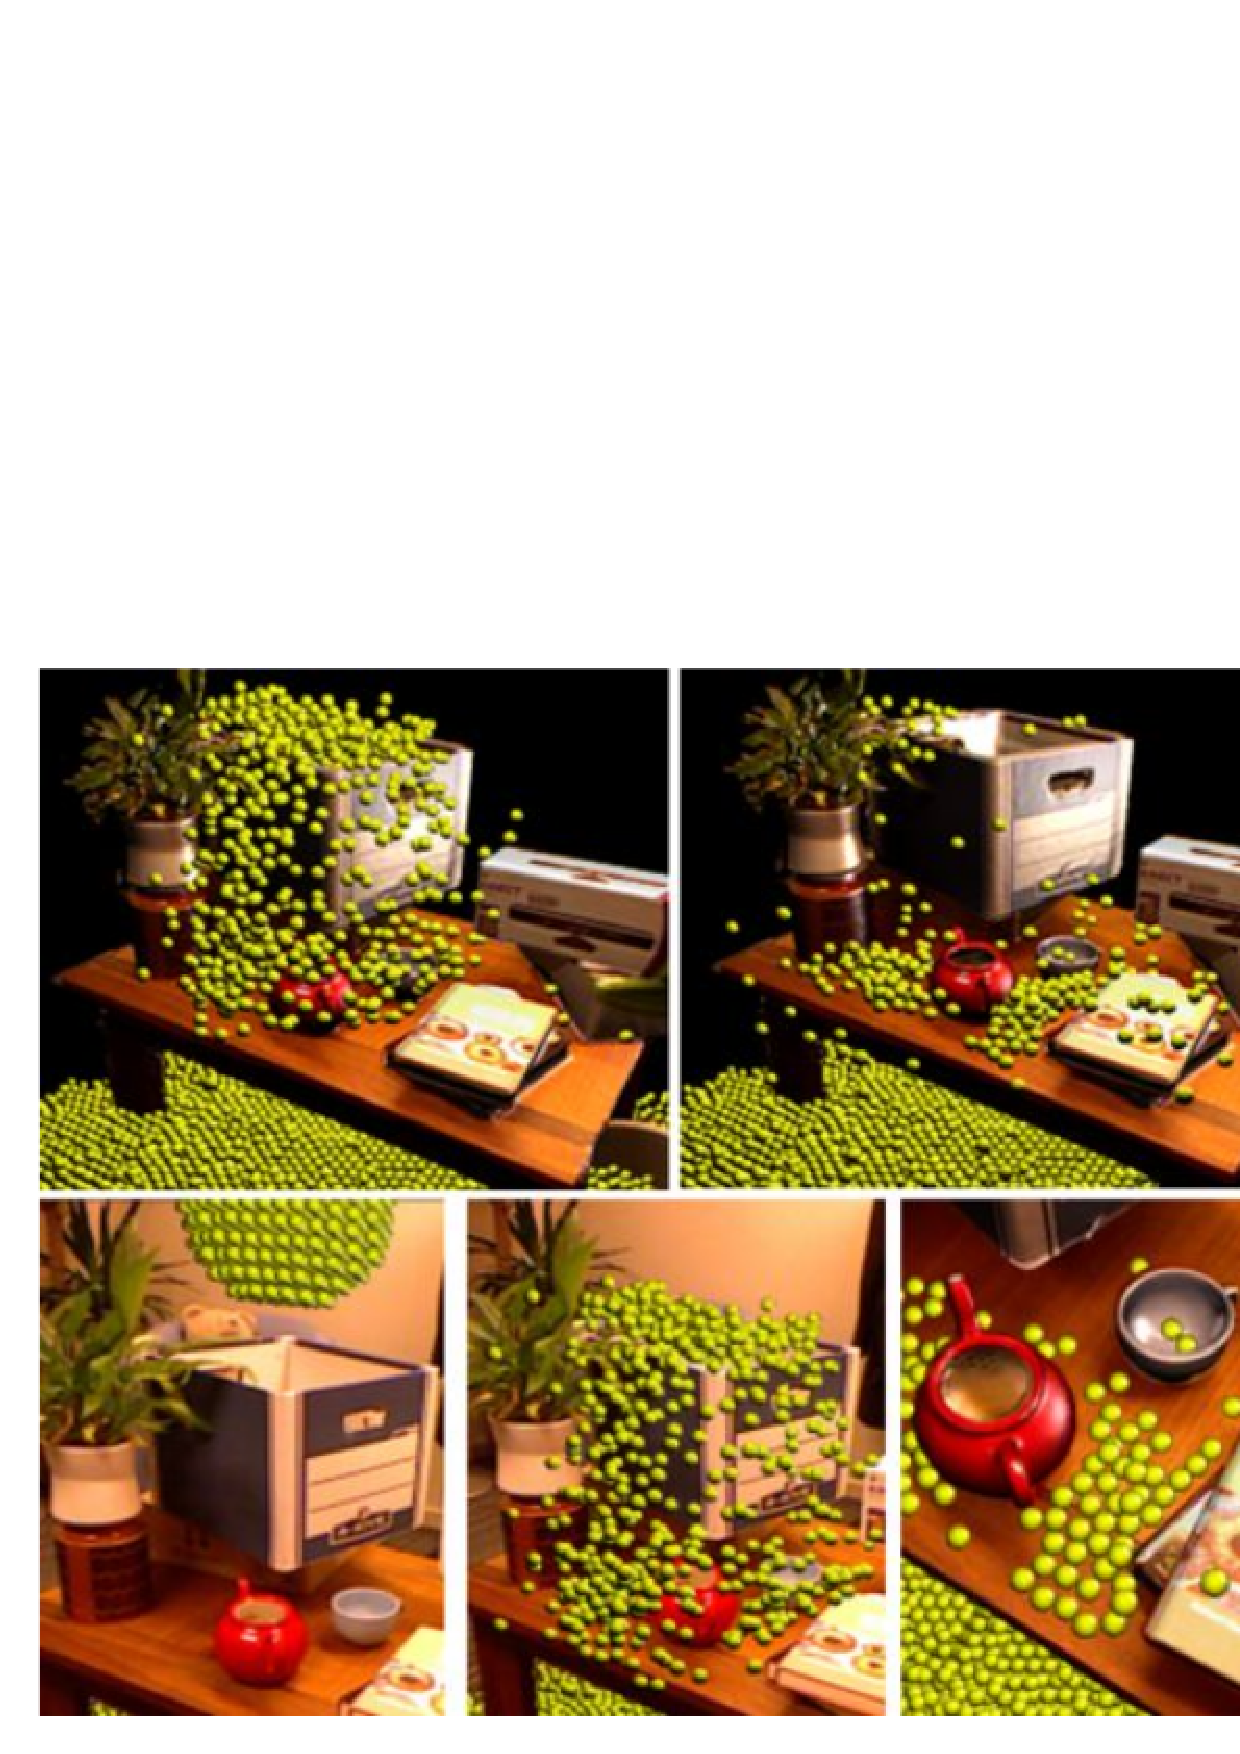
\includegraphics[scale=0.34]{images/izadi}
\caption{Reconstructed 3D scene with thousands of virtual particles.}
\label{fig:izadi}
\end{center}
\end{figure}


%done
In \cite{keqiang} a 3D reconstruction is performed with a laser range finder (SICK 2D) and a mobile robot, 
using the ICP algorithm and a volumetric representation. In the matching phase of the ICP algorithm not all
 points are used, instead they just use edge points, reducing the computational cost of the process. The scene 
 representation is simplified removing redundant points, this is done dividing the scene into voxels and at each 
 voxel preserving just the point closer to the center. Their system produces a scene with data points evenly 
 distributed.

%similar work
Point cloud registration using 3D edges is used in \cite{choi13}. The edges are obtained working in the depth map and the RGB image, 
using 8-neighbor search in a 2D image to obtain four different types of edges. Geometric and photometric information is used to 
obtain edges and then ICP algorithm is used to perform the point cloud alignment.  

%similar work2

Another work using edges in combination with ICP is \cite{dryan2012}. Where also a combination of RGB and depth map information is 
used. They detect edges converting RGB image to grayscale and applying Canny edge detector. Then points are extracted from 
the depth map to obtain 3D points. A filtering is made, to discard edges produced in the background of an object near object borders. 
Then ICP algorithm is applied over this subset, applying a rejection method based on the edge orientation in the image space. Finally, 
they apply the ICP algorithm over the entire point cloud to refine the transformation.

%new 
Point cloud registration using features extracted from the RGB image is used in \cite{endres13}. Their algorithm uses visual features 
backprojected to 3D points in order to align the point clouds. They use graph optimization to reduce drift error and they propose a 
transformation verification method independent of the used estimation method, using the free-space information,
exploiting the availability of structured dense data they use a beam-based Environment Measurement Model (EMM). That basically consists 
in applying the transformation founded with their method to the point cloud and the projecting the 3D points to the target depth map, 
to verify if there is consistency 
between the transformed point cloud and the target point cloud depth map.


Most methods combine visual and geometrical information when both types of data are available. There is not a method 
that adapts to all possible scenarios. Most methods assume a static scene and lambertian 
surfaces. For this reason, some materials such as glass or water can ruin the reconstruction. 
Depending on the requirements one method can be preferred 
over another, sometimes computational efficiency is more important than reconstruction quality or vice versa.










